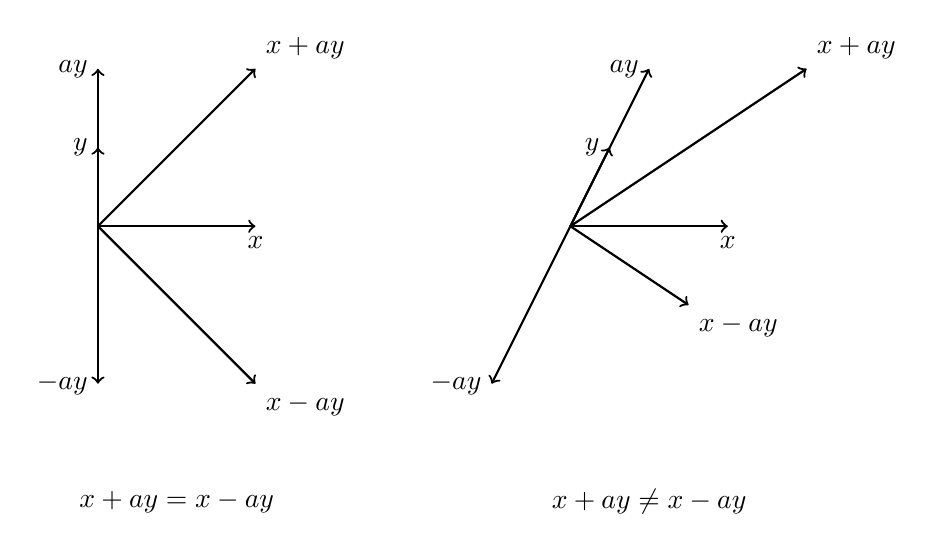
\begin{tikzpicture}
    % Left Diagram
    \draw[thick,->] (0,0) -- (2,0) node[below] {$x$};
    \draw[thick,->] (0,0) -- (0,1) node[left] {$y$};
    \draw[thick,->] (0,0) -- (0,2) node[left] {$a y$};
    \draw[thick,->] (0,0) -- (0,-2) node[left] {$-a y$};
    \draw[thick,->] (0,0) -- (2,2) node[above right] {$x + a y$};
    \draw[thick,->] (0,0) -- (2,-2) node[below right] {$x - a y$};
    
    % Right Diagram
    \begin{scope}[xshift=6cm]
        \draw[thick,->] (0,0) -- (2,0) node[below] {$x$};
        \draw[thick,->] (0,0) -- (.5,1) node[left] {$y$};
        \draw[thick,->] (0,0) -- (1,2) node[left] {$a y$};
        \draw[thick,->] (0,0) -- (-1,-2) node[left] {$-a y$};
        \draw[thick,->] (0,0) -- (3,2) node[above right] {$x + a y$};
        \draw[thick,->] (0,0) -- (1.5,-1) node[below right] {$x - a y$};

    \end{scope}
    
    % Bottom equations
    \node at (1,-3.5) {$\norm{x + ay} = \norm{x - a y}$};
    \node at (7,-3.5) {$\norm{x + a y} \neq \norm{x - a y}$};
\end{tikzpicture}